% !TEX encoding = UTF-8 Unicode

\documentclass[twocolumn,10pt,a4j]{ltjsarticle}
\usepackage{kougai}

\title{VRコンテンツにおける人体表現の違和感について}
\author{2132086 谷 祥英  指導教員 須田 宇宙 准教授}
\date{}

\begin{document}

\maketitle

\section{はじめに}
  VRは知覚を模倣した情報呈示により3DCG空間を現実のように体験でき,教育や医療,エンターテインメントなど多岐にわたり利用されている.
  近年では3Dモデルやモーションデータの共有プラットフォームを利用した,3DCGによるVRコンテンツ制作が広く行われている.

  VRに限らず,様々なコンテンツ内で人体表現は誘目性が高い.VRコンテンツにおける人体表現では,CGキャラクターとその動きが主な要素として挙げられる.
  しかし,VR体験中に人体表現に違和感を覚えることが少なくないことが問題である.

  そこで本研究では,VRコンテンツにおける人体表現の違和感について調査することを目的とする.

\section{3DCGの違和感と両眼視差の心理的影響}
  ロボット工学や3DCGなどの分野では,人体やその動作のリアリティの向上に伴い親和感も向上するが,ある区間では親和感が急激に落ち込むとされる,不気味の谷現象の実証的研究が広く行われている\cite{Uncanny}.
  親和感の逆を違和感であると仮定した場合に,あるリアリティの区間では違和感が急激に増加する傾向があるといえる.

  質感の知覚は,物の美醜など印象に影響する要素の一つである.
  両眼視差式の3D画像による質感の知覚は2D画像によるものと異なることが報告されている\cite{VR_texture}.
  VRでは両眼視差式の立体映像が呈示されることが多く.3DCGによる表現から受ける印象は平面映像のものと同一ではないことが考えられる.

  これらのことから,3DCGによるVRコンテンツの人体表現の違和感は,不気味の谷のような傾向を示すが,2D映像のものとは異なることが考えられる.

\section{調査概要}
  本研究では,CGキャラクターのリアリティによる違和感への影響に着目し,広範に制作されるVRコンテンツにおける人体表現の違和感について調査することを目的とした.
  コンテンツ共有プラットフォームから利用できる複数のCGキャラクターと単一のモーションデータから映像を作成し,立体映像のの主観評価実験を行った.

  リアリティについて,(a)キャラクター的であるかと(b)現実的であるかの2項目について,1.全く当てはまらない,2.当てはまらない,3.あまり当てはまらない,4.やや当てはまる,5.当てはまる,6.よく当てはまるの6段階による評価を調査した.
  違和感について,(c)違和感の有無と,その詳細を聴取した.
  
  (a)と(b)の相関関係を図\ref{fig1}に示す.2項目間の相関係数は-0.998で強い負の相関がみられ,リアリティにおいてキャラクター的であるかと現実的であるかは対立した評価語であることが分かった.リアリティの評価は青色で示した高群と橙色で示した低群の,大きく2群に分かれた.
   
  \begin{figure}[H]
    \centering
    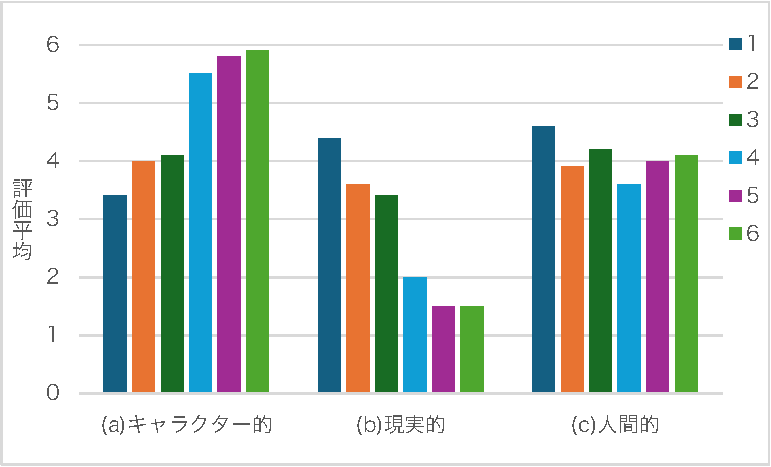
\includegraphics[width=\linewidth]{fig1.pdf}
    \caption{(a)キャラクター的であるかと(b)現実的であるかの評価の相関関係\label{fig1}}
  \end{figure}

  各映像で違和感を覚えた被験者の割合を,リアリティについて降順で図\ref{fig2}に示す.
  リアリティの評価の高郡を青色,低郡を橙色で示している.
  (a)と(c)の相関係数は-0.375で中程度の負の相関が,(b)と(c)の相関係数は0.405で中程度の相関がみられたことから,リアリティの高い映像に違和感を覚えやすいことが示唆された.
  
  \begin{figure}[H]
    \centering
    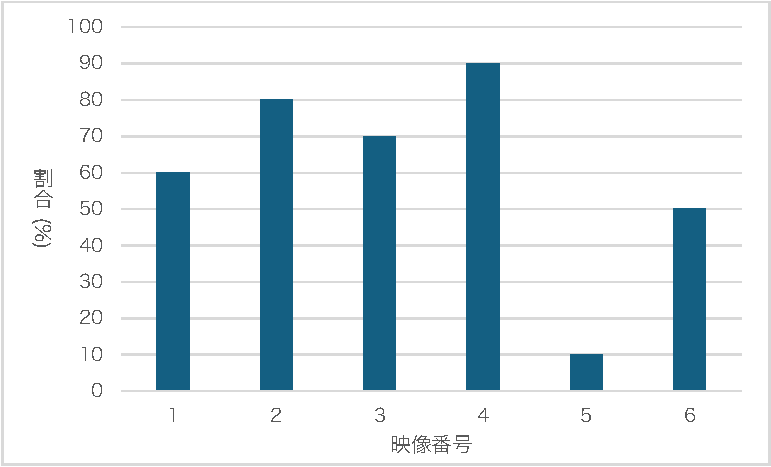
\includegraphics[width=\linewidth]{fig2.pdf}
    \caption{違和感を覚えた被験者の割合\label{fig2}}
  \end{figure}
  
\section{終わりに}
  調査結果から,CGキャラクターのリアリティの高い映像に違和感を覚えやすいことが示唆された.
  本研究ではCGキャラクターを中心とした調査を行ったが,今後アニメーションを中心とした調査も行い違和感について検討していく必要がある.

\begin{thebibliography}{99}
  \bibitem{Uncanny}森 政弘.(1970) 不気味の谷. Energy. 7(4), 33-35.
  \bibitem{VR_texture}尾島 修一, 植村 匠.(2014) 両眼視差が光沢感に与える影響についての一実験. 平成26年度電気・情報関係学会九州支部連合大会講演論文集. 334.

\end{thebibliography}

\end{document}
